\section{Implementation and Encountered Problems}

In this section, we present our implementation choices and compare them to discarded alternatives to justify them. 
We also describe what difficulties we encountered during development and how we addressed them.

\subsection{Syntax}

First, we formalize the abstract syntax of boolean formulas containing conjunctions, disjunctions, implications, and negations. 

\subsubsection{Abstract Syntax.}

We state an inductive definition of the type \texttt{form} with a set of constructors describing how to build up a formula:
\begin{equation}
    p, q ::= x\;|\;\texttt{true}\;|\;\texttt{false}\;|\;p \land q\;|\;p \lor q\;|\;p \rightarrow q\;|\;\neg p
\end{equation}

For identifiers, we introduce the type \texttt{id} with a single constructor \texttt{Id} that wraps a string. We also define an equality function comparing two identifiers and returning \texttt{true} if and only if their contained strings are equal. To ease proof development in the rest of the project, we prove some basic lemmas about the function by case distinction, namely \emph{reflexivity}, \emph{equivalence with propositional equality}, and \emph{decidability} of equality of identifiers.

\subsubsection{Concrete Syntax.}

To make reading and writing formulas easier, we use \textsc{Coq}'s \texttt{Notation}s system, as well as a \texttt{Coercion} from an identifier as a formula. 
The main difficulty lies in assigning precedence levels to the individual constructors that pay respect to the commonly assumed binding of operators. 
Given the \emph{binds stronger} relation ($>$), that is:
\begin{equation}
    \neg > \land > \lor >\,\rightarrow
\end{equation}
For example, $x \lor \neg y \land z \rightarrow \texttt{false}$ is interpreted as $(x \lor ((\neg y) \land z) \rightarrow \texttt{false}$. 

\subsection{Semantics}

Now that we can write a formula in \textsc{Coq}, we want to define its semantics, i.e., if we interpret it as \texttt{true} or \texttt{false}.

\subsubsection{Valuations.}

To do so, we need to know which boolean values to replace all identifiers occurring in a formula with.
Therefore, we define the type \texttt{valuation}. 
A valuation is a function that, being passed an identifier, returns \texttt{true} or \texttt{false}, or, in other words, a valuation is a total map from identifiers to booleans. Our implementation is analogous to the total map defined by Pierce et al. in \cite{pierceSF}.
% An empty valuation is a valuation that returns \texttt{false} for all arguments.

Again, to simply writing and reading valuations, we introduce a \textsc{Notation} \texttt{x !-> b ;; v} to override a valuation \texttt{v} with a new value \texttt{b} for \texttt{x}. At first, we used just a single semicolon, but this causes conflicts with list notations. 

We also specify some lemmas of \cite{pierceSF} for later reasonings. Their proofs rely on the functional extensionality axiom, stating that two functions are equal if and only if their applications to all their possible arguments are equal. It is known to be compatible with \textsc{Coq}'s logical core.

\subsubsection{Interpreter.}

The \texttt{valuation} type allows us to define a recursive interpreter function.
Applied to a valuation and a formula, it returns \texttt{true} if and only if the formula holds by traversing a formula bottom-up and pattern matching on it.
All the necessary functions, such as \texttt{andb}, \texttt{orb}, and \texttt{negb} are already implemented in \textsc{Coq}. 
They even suffice to compute the result of an implication since $p \rightarrow q$ is known to be equivalent to $\neg p \lor q$.

\subsection{Optimizer}

\subsection{A Subsection Sample}
Please note that the first paragraph of a section or subsection is
not indented. The first paragraph that follows a table, figure,
equation etc. does not need an indent, either.

Subsequent paragraphs, however, are indented.

\subsubsection{Sample Heading (Third Level)} Only two levels of
headings should be numbered. Lower level headings remain unnumbered;
they are formatted as run-in headings.

\paragraph{Sample Heading (Fourth Level)}
The contribution should contain no more than four levels of
headings. Table~\ref{tab1} gives a summary of all heading levels.

\begin{table}
\caption{Table captions should be placed above the
tables.}\label{tab1}
\begin{tabular}{|l|l|l|}
\hline
Heading level &  Example & Font size and style\\
\hline
Title (centered) &  {\Large\bfseries Lecture Notes} & 14 point, bold\\
1st-level heading &  {\large\bfseries 1 Introduction} & 12 point, bold\\
2nd-level heading & {\bfseries 2.1 Printing Area} & 10 point, bold\\
3rd-level heading & {\bfseries Run-in Heading in Bold.} Text follows & 10 point, bold\\
4th-level heading & {\itshape Lowest Level Heading.} Text follows & 10 point, italic\\
\hline
\end{tabular}
\end{table}


\noindent Displayed equations are centered and set on a separate
line.
\begin{equation}
x + y = z
\end{equation}
Please try to avoid rasterized images for line-art diagrams and
schemas. Whenever possible, use vector graphics instead (see
Fig.~\ref{fig1}).

\begin{figure}
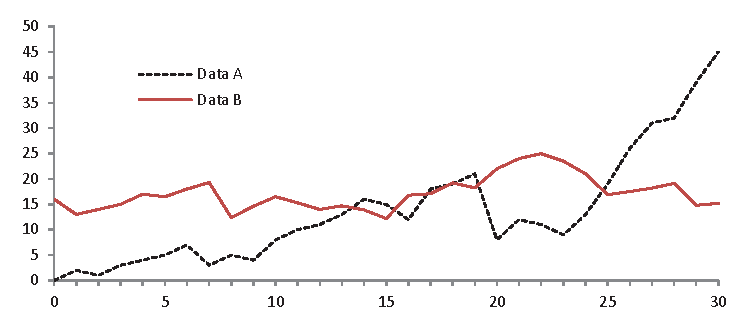
\includegraphics[width=\textwidth]{fig1.eps}
\caption{A figure caption is always placed below the illustration.
Please note that short captions are centered, while long ones are
justified by the macro package automatically.} \label{fig1}
\end{figure}

\begin{theorem}
This is a sample theorem. The run-in heading is set in bold, while
the following text appears in italics. Definitions, lemmas,
propositions, and corollaries are styled the same way.
\end{theorem}
%
% the environments 'definition', 'lemma', 'proposition', 'corollary',
% 'remark', and 'example' are defined in the LLNCS documentclass as well.
%
\begin{proof}
Proofs, examples, and remarks have the initial word in italics,
while the following text appears in normal font.
\end{proof}
For citations of references, we prefer the use of square brackets
and consecutive numbers. Citations using labels or the author/year
convention are also acceptable. The following bibliography provides
a sample reference list with entries for journal
articles~\cite{ref_article1}, an LNCS chapter~\cite{ref_lncs1}, a
book~\cite{ref_book1}, proceedings without editors~\cite{ref_proc1},
and a homepage~\cite{ref_url1}. Multiple citations are grouped
\cite{ref_article1,ref_lncs1,ref_book1},
\cite{ref_article1,ref_book1,ref_proc1,ref_url1}.